\section{A First Trivial Approach using Merge Sort}
\label{tree:xy:merge}

\begin{figure}
\centering
\begin{subfigure}[b]{0.40\textwidth}
\centering
	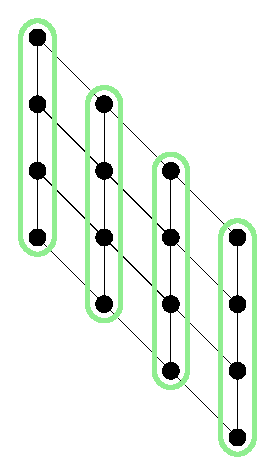
\includegraphics[width=0.4\textwidth]{fig/x+y/poset/chains}
	\caption{Balanced selection of disjoint chains in the \XY poset.}
	\label{fig:xy:poset:chains}
\end{subfigure}
\begin{subfigure}[b]{0.40\textwidth}
\centering
	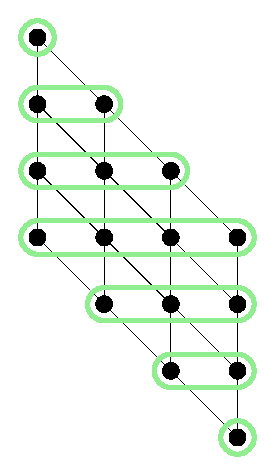
\includegraphics[width=0.4\textwidth]{fig/x+y/poset/antichains}
	\caption{Maximal antichains in the \XY poset.}
	\label{fig:xy:poset:antichains}
\end{subfigure}
\caption{Structure of the \XY poset.}
\label{fig:xy:poset:diagrams}
\end{figure}

\begin{figure}
\centering
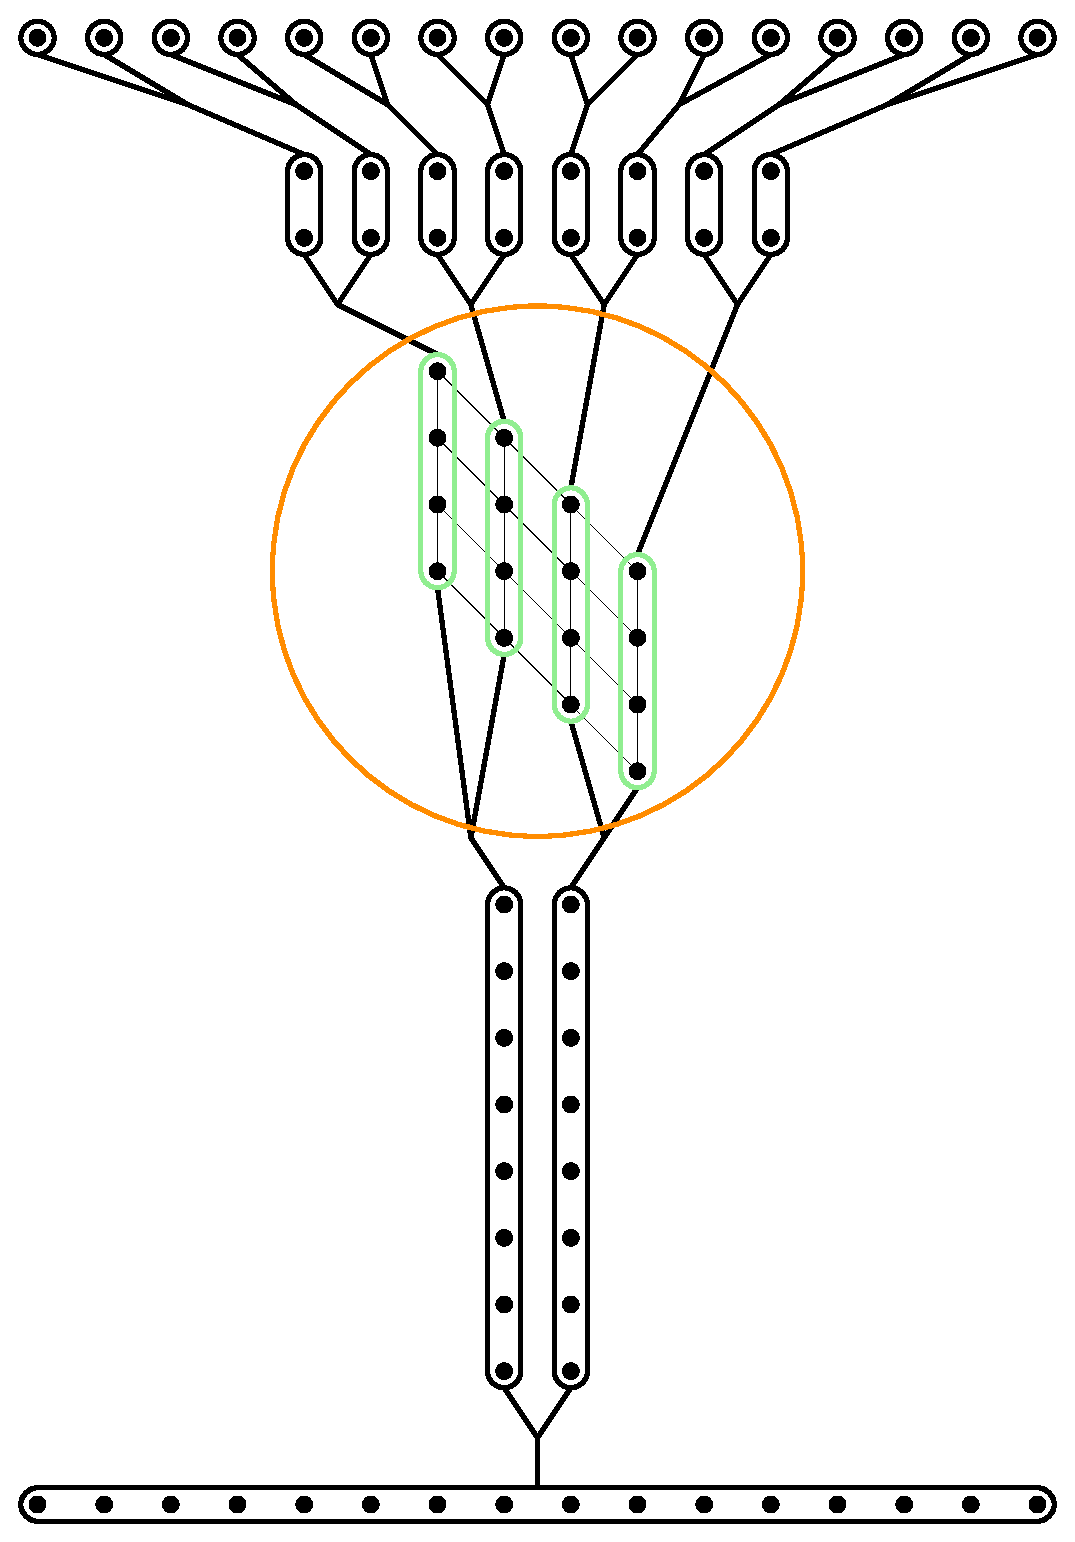
\includegraphics[width=0.5\textwidth,angle=90]{fig/x+y/poset/mergexy}
\caption{Resolution of the Mergesort algorithm with the part
corresponding to the starting point of a sort \XY problem highlighted.}
\label{fig:xy:poset:mergexy}
\end{figure}

We define the poset structure of \XY (or simply the \XY poset) to be the poset
containing the information that we can extract from the transitivity of the
total order on \(X \cup Y\). If we only exploit the fact that
\(X_i \le X_{i'} \land Y_j \le \Y_{j'} \implies X_i + Y_j \le X_{i'} + Y_{j'}\)
we obtain the posets represented by the Hasse diagrams (\ref{tree:poset:hasse})
in \ref{fig:xy:poset:diagrams}.

In this first, trivial attempt, we will use the poset structure on the elements
in \XY to reduce by a factor of $2$ the number of comparisons
required to sort \XY compared to the execution of the Mergesort algorithm
without knowledge of this structure.

In \ref{tree:related:xy} we saw \ref{fig:related:xy} which shows us all the order
relations between elements of \XY. Now, we will see that chains and antichains
in \XY obey a regular pattern. To illustrate this, we take the $4 \times 4$
\XY problem. We highlight a possible selection of disjoint chains in
\ref{fig:xy:poset:chains} and the set of maximal antichains in
\ref{fig:xy:poset:antichains}.

Now we will solve this problem in a strictly faster way than sorting all
of its elements, by taking advantage of some of the information we already have.

First, we show that sorting \XY without information using the merge sort algorithm would use $2
n^2 \log n$ comparisons. The exact upper bound on the number
of comparisons required to solve an instance of size \(N\) with this algorithm
is given by the formula
\begin{align*}
T(N) &= N - 1 + T(\floor{\sfrac{N}{2}}) + T(\ceil{\sfrac{N}{2}})\\
T(0) &= T(1) = 0.
\end{align*}
Note that there is a non recursive way to express \(T(N)\) (\citet*{OEIS:A001855}) which is
\begin{displaymath}
T(N) = \sum_{k=1}^{N} \ceil{\log k}.
\end{displaymath}
We have
\begin{displaymath}
\lim_{N\to\infty}\frac{T(N)}{\log N!} =
\lim_{N\to\infty}\frac{\sum_{k=1}^{N}\ceil{\log k}}{ \sum_{k=1}^{N} \log k} = 1
\end{displaymath}
and thus, by Stirling's approximation, the merge sort algorithm requires at
most \(N \log N\) comparisons for very large \(N\). When we sort \XY, we have \(N =
n^2\), and thus
\[N \log N = n^2 \log n^2 = 2 n^2 \log n.\]
Indeed, we give here an example where \(n\) is a power of \(2\) but it is not
difficult to convince oneself that for very large \(n\) the complexity added
by the ceiling and flooring functions fade away.

We now show that it is possible to sort \XY with half the comparisons. The
merge sort algorithm has this particularity that at the end of every step of
the recursion we are left with several total orders on disjoint subsets of the
set to sort. To illustrate, if we organise steps in stages we obtain what is
shown in \ref{fig:xy:poset:mergexy}.

What is highlighted in \ref{fig:xy:poset:mergexy} is a subset of the
information we have when knowing the structure of \XY, \ie the chains of
\ref{fig:xy:poset:chains}. It means that the stage we
highlighted can be attained without any comparison if the set to sort is \XY
and if we know its structure. Note that if not known a priori, this structure
can be revealed for the cost of \(2n \log n\) comparisons, using a standard \(n
\log n\) comparison sorting algorithm to sort sets \(X\) and \(Y\).

Remember that in merge sort there are $\log N$ stages. At stage $i$ we have
built $2^{i}$ total orders on disjoint subsets of size $2^{\log N - i}$. Since
the stage represented in \ref{fig:xy:poset:mergexy} shows $n$ total orders on
disjoint subsets of size $n$, and that the total number of elements in $X+Y$ is
$N = n^2$ we can conclude that \ref{fig:xy:poset:mergexy} shows us step
$\sfrac{1}{2} \log N$. It should be possible to prove from scratch that
starting the algorithm at the median step saves us half the comparisons, for
\(n\) large enough. However we will rely on the results we gave
in \ref{tree:merging:kgeq3} to prove that it is indeed the case.

\begin{proof}
Note that if \(2n^2 \log n\) is the total amount of information to retrieve,
then recycling the information contained in the \(n\) chains of length \(n\)
gives us \(n \cdot n \log n = n^2 \log n\) bits of information already in our
possession. We already saw that we can reuse this information optimally using
the Huffman code based merging algorithm.
\end{proof}

Since this algorithm reuses only a fraction of the available information, the
question of the optimality of this approach remains. This question will be
answered in the next section.
